% pdfLaTeX. Complete IEEE journal first draft, October 26, 2026.
% Author order retained from the supplied VBC/IBC manuscript for coauthor confirmation.
% All degree bounds mean total degree at most the prescribed d.
\documentclass[journal,10pt]{IEEEtran}
\usepackage[T1]{fontenc}


\usepackage{amsmath,amssymb,amsthm,booktabs,array,microtype}
\usepackage{needspace,graphicx,cite}
\usepackage[dvipsnames]{xcolor}
\usepackage[colorlinks=true,linkcolor=MidnightBlue,urlcolor=MidnightBlue,citecolor=MidnightBlue]{hyperref}
\newtheorem{theorem}{Theorem}
\newtheorem{lemma}{Lemma}
\newtheorem{proposition}{Proposition}
\newtheorem{corollary}{Corollary}
\theoremstyle{definition}\newtheorem{definition}{Definition}
\theoremstyle{remark}
\newtheorem*{remark}{Remark}
\newcommand{\R}{\mathbb R}
\newcommand{\co}{\operatorname{conv}}
\newcommand{\cl}{\operatorname{cl}}
\newcommand{\dist}{\operatorname{dist}}
\newcommand{\one}{\mathbf 1}
\newcommand{\ball}{\mathbb B_V}
\newcommand{\F}{\mathcal F_d}
\newcommand{\K}{\mathcal K_\varepsilon}
\newcommand{\dd}{\,\mathrm d}

\hypersetup{pdftitle={Structural Conservatism of Discrete-Time Barrier Certificates: Moment Obstructions and Degree Separations},pdfauthor={Reza Iraji, Vishnu Murali, and Majid Zamani}}
\title{Structural Conservatism of Discrete-Time Barrier Certificates:
Moment Obstructions and Degree Separations}
\author{Reza Iraji, Vishnu Murali, and Majid Zamani%
\thanks{The authors are with the Department of Computer Science, University of Colorado Boulder, Boulder, CO 80309, USA. Corresponding author: Reza Iraji (email: reza.iraji@colorado.edu).}}
\markboth{Author Review Draft, October 2026}{Iraji et al.: Structural Conservatism of Discrete-Time Barrier Certificates}
\begin{document}
\maketitle
\begin{abstract}
Increasing polynomial degree and adding certificate functions address different restrictions in safety verification. For autonomous discrete-time systems, we study fixed-anchor vector barrier certificates with constant nonnegative comparison matrices and interpolation-inspired certificates with implication propagation. A truncated-moment criterion excludes every finite number of vector components at a prescribed degree. A fixed-family characterization identifies the underlying convexified averaging requirement. A converse characterizes prescribed-degree forward certificates with Schur-stable matrices by robust separation of the convexified monomial dynamics, including independent source and successor errors. From a supplied, certified convex body, classical approximation and finite linear programs extract finitely many functions and a global matrix with explicit error budgets. A nonlinear family has minimum implication-certificate degree two and minimum comparison degree four, in either direction. A different cubic family has minimum forward scalar comparison degree two but minimum finite-vector degree one. Exact rational evidence verifies the examples. The results distinguish settings where more functions suffice from settings where every same-degree refinement fails. Ordinary certificates with spectral radius one remain outside the Schur-stable converse.
\end{abstract}
\begin{IEEEkeywords}
Safety verification, barrier certificates, invariant sets, polynomial methods, moment obstructions, positive systems.
\end{IEEEkeywords}

\section{Introduction}
\IEEEPARstart{S}{afety} verification asks whether a dynamical system can reach an unsafe set from specified initial states. Barrier certificates answer this question through inequalities rather than explicit reachable-set computation. Polynomial templates enable optimization, but an unsuccessful search does not identify its cause. Degree, function count, propagation conditions, the verification domain, and the chosen relaxation can each restrict feasibility.

Vector barrier certificates (VBCs) compare several functions through a nonnegative matrix, whereas interpolation-inspired barrier certificates (IBCs) propagate a finite sequence of sublevel sets \cite{vector,ibc,submission}. Adding components refines an invariant without necessarily increasing its degree. However, a global constant comparison also holds after averaging source and successor values. An implication rule need only constrain actual transitions from an active antecedent set. This raises a formulation-selection question: at a fixed degree, can additional functions repair a certificate, or must its degree or propagation conditions change?

We study existence, rather than interpreting solver failure as nonexistence. Our scope is autonomous deterministic discrete-time safety, with a fixed unsafe anchor in the forward VBC class. This restriction is essential for the general moment obstruction. The backward class reverses endpoint separation and the comparison inequality; the robust converse concerns only the forward class.

The contributions are:
\begin{enumerate}
\item A prescribed-degree moment criterion excludes every finite component count and every constant nonnegative comparison matrix, in either direction. A fixed-family characterization explains the averaging requirement through classical convex duality.
\item Robust separation of the full convexified monomial relation is equivalent to a finite prescribed-degree forward VBC with strict global propagation, and to an ordinary VBC with $\rho(A)<1$. Transition pairs and reachable feature sets are both convexified.
\item From a supplied, certified convex body, finite facets and row LPs extract a certificate with explicit source/successor error budgets. The sharper geometric exponent is classical Dudley approximation. The method does not discover the body automatically.
\item Two exact degree comparisons separate propagation rules from function count. One nonlinear family has minimum implication-IBC degree two and minimum fixed-anchor comparison degree four, allowing arbitrary finite counts and either direction. A different cubic family has minimum forward scalar comparison degree two and minimum finite-vector degree one: every scalar affine comparison fails and four affine components suffice.
\end{enumerate}
The general neutral-class converse, automatic body discovery, and minimum component counts remain future work. The examples use exact rational proof data.

\section{Certificate Classes and Scope}\label{sec:classes}
Consider $x^+=f(x)$, where $X\subseteq\R^n$ is nonempty and compact, $f:X\to X$ is continuous, and $X_0,X_u\subseteq X$ are nonempty, compact and disjoint. Safety means $f^k(X_0)\cap X_u=\varnothing$ for every integer $k\geq0$. Vector inequalities are componentwise, $A\geq0$ is entrywise nonnegative, and degree means total degree at most a prescribed $d\geq1$.

\begin{definition}[Fixed-anchor comparison VBCs]\label{def:vbc}
A forward certificate consists of a finite polynomial vector $B=(B_1,\ldots,B_m)^\top$, a constant $A\geq0$, and $\delta_0,\delta_u>0$ such that
\begin{equation}\label{eq:ordinary}
\begin{aligned}
 B&\leq-\delta_0\one &&\text{on }X_0,\\
 B_1&\geq\delta_u &&\text{on }X_u,\\
 B\circ f&\leq AB &&\text{on }X.
\end{aligned}
\end{equation}
A backward certificate instead satisfies
\begin{equation}\label{eq:backward}
\begin{aligned}
 B&\leq-\delta_u\one &&\text{on }X_u,\\
 B_1&\geq\delta_0 &&\text{on }X_0,\\
 B(x)&\leq AB(f(x)) &&(x\in X).
\end{aligned}
\end{equation}
No spectral restriction is part of the definition.
\end{definition}
The fixed anchor is stronger than pointwise unsafe separation, which permits the positive component to depend on the unsafe state. The general moment obstruction is not claimed for that broader class.

\begin{definition}[Implication IBCs]\label{def:ibc}
For finitely many polynomial frames put $s(i)=\min\{i+1,m\}$. A forward IBC has $b_1\leq0$ on $X_0$, every $b_i>0$ on $X_u$, and
\[
 b_i(x)\leq0\ \Longrightarrow\ b_{s(i)}(f(x))\leq0\quad(x\in X).
\]
A backward IBC has $b_1\leq0$ on $X_u$, every $b_i>0$ on $X_0$, and
\[
 b_i(f(x))\leq0\ \Longrightarrow\ b_{s(i)}(x)\leq0\quad(x\in X).
\]
One frame is permitted.
\end{definition}
These are the implication conditions in \cite{ibc,submission}. Globally scaled IBCs are a stronger class; for example their forward propagation is $\lambda_i b_{s(i)}\circ f\leq b_i$ on all of $X$ for positive constants $\lambda_i$, together with the endpoint margins in \cite{submission}. We do not identify this stronger class with implication IBCs.

\begin{proposition}[Soundness]
Either comparison direction and either implication direction imply safety.
\end{proposition}
\begin{proof}
Forward comparisons give $B(f^k(x_0))\leq A^kB(x_0)\leq0$, excluding the unsafe anchor. A backward-certified trajectory reaching $x_k\in X_u$ would give $B(x_0)\leq A^kB(x_k)\leq0$, contradicting the initial anchor. A forward IBC gives $b_{\min\{k+1,m\}}(x_k)\leq0$ by induction. A backward IBC starts at $b_1(x_k)\leq0$ and iterates backward along the finite trajectory, contradicting positivity on $X_0$.
\end{proof}

\section{Relation to Prior Work}\label{sec:literature}
\subsection{Increment over the group papers}
The submitted VBC/IBC paper \cite{submission} proves degree- and count-preserving correspondence between globally scaled IBCs and weighted-path VBCs, exchanging direction and sign. It also proves affine separations using rotations and a nonlinear scalar example. We retain its definitions and credit those mechanisms; neither path/scaled correspondence nor cyclic coupling is a new claim here.

Theorem 9 of \cite{submission} uses a convexified affine transition pair in $X_0\times X_u$ to exclude affine VBCs even under pointwise endpoint separation. Our moment theorem permits distributed endpoint measures and any prescribed degree. This generality requires the fixed anchor, since averaging different pointwise-positive components need not preserve one positive average. Point-mass endpoints at degree one recover the earlier affine mechanism.

The nonlinear example in \cite{submission} has minimum implication degree one and only $2\leq d_{\rm VBC}^{\min}\leq4$. Our distinct symmetric example excludes every comparison VBC through degree three, proving minima two and four over an open parameter region. The cubic family separately extends the rotation mechanism to a perturbation neighborhood and proves an exact scalar/vector degree tradeoff.

The IBC construction \cite{ibc} combines finite frames but does not provide the component-count-independent moment exclusion proved here. Path-complete barriers \cite{anand} concern graph soundness and ordering for switched safety. Path-complete closure certificates \cite{pccc} use relational functions for persistence under switching. Those graph and persistence guarantees are not transferred to the present state-function safety setting.

\subsection{Theorem~\ref{th:main}: the existence equivalence}
\textbf{Closest multiplier result: Horv\'ath--Song--Terlaky, Theorem 3.10 and Remark 3.11.}
For a supplied convex function $g$ and its sublevel set $\{g\leq0\}$, \cite{hst} assumes
strict feasibility and concavity of $g\circ f_d$, and characterizes its
invariance by $g\circ f_d\leq\lambda g$ globally on $\R^n$, for
$\lambda\geq0$. If both functions are quadratic, the S-lemma removes the
successor-concavity assumption; Remark 3.11 extends the first statement
to several convex inequalities.
Our Lemma~\ref{lem:dual} is the same classical duality mechanism on a compact
convex relation. Theorem~\ref{th:main} instead starts with no supplied
polynomial family, assumes positive-radius separation after full graph and
reachable-set convexification in a fixed feature space, and concludes existence
of finitely many degree-bounded functions with a designated unsafe anchor and
$\rho(A)<1$, together with the converse implication.
No concavity of $B_i\circ f$ is required, but ordinary state-space invariance
has been replaced by a stronger convexified-feature robustness condition.
Thus the theorem is not an unconditional removal of their concavity assumptions.

\textbf{Closest smooth safety converse: Liu, Section IV, Theorem 30.}
The discrete-time result in \cite{liu} uses additive state-disturbance robust
safety, separation of the disturbed reachable closure from the unsafe set,
local Lipschitz regularity, and compactness of that closure or global
Lipschitz continuity. It gives a smooth robust barrier at a smaller disturbance
radius. Our hypothesis uses independent feature errors and convexified
transition pairs; our conclusion prescribes the polynomial degree and a
constant nonnegative Schur comparison. Section~\ref{sec:physical} proves
that physical robustness alone need not satisfy this feature premise.
Neither converse subsumes the other through a simple change in disturbance radius.

\textbf{Closest polynomial-cone/positive-system result: Berger--Ghanbarpour--Sankaranarayanan, HSCC 2024.}
Theorem 3.5 of \cite{cone2024} proves invariance for polynomial ODEs from
$L_f(g)+\lambda g\in\operatorname{cone}(K G^{\leq\ell})$, using positive
systems. Definition 5.1 and Corollary 5.2 turn this sufficient condition into
a refinement fixed-point criterion. It permits polynomial multipliers and
products of generators, and already uses polynomial templates and multiple
inequalities. Our constant-matrix coupling is more restricted. Our equivalence concerns
robust convexified fixed-feature separation with an unsafe anchor and Schur scope.
Neither polynomial features, positive comparison systems, nor cone refinement
is claimed new here.

\subsection{Theorem~\ref{th:count} and Proposition~\ref{prop:projection}: conditional facets}
\textbf{Closest geometry: Har-Peled--Jones, Theorem 1.4.}
The classical Dudley result in \cite{harpeled} approximates a supplied bounded
convex body by $O_r((R/\tau)^{(r-1)/2})$ supporting halfspaces within
Hausdorff error $\tau$. Proposition~\ref{prop:projection} applies this mechanism
with a prescribed unsafe separator, explicit support/projection-gap error
budgets, and $\tau=\varepsilon/2$. The exponent is classical.
Theorem~\ref{th:count} gives a coarser direct support-net alternative.
The degree bound comes from composing affine facets with the fixed feature map,
not from a new convex approximation theorem.

\textbf{Closest dynamical approximation: Alessio--Lazar--Bemporad--Heemels, Theorem 4.}
Theorem 4 in \cite{alessio} is a general intermediate-set inclusion result for
perturbed nonlinear discrete-time dynamics: an approximation within a
contraction margin preserves the corresponding invariance/contraction property.
Ellipsoids enter its later finite construction, not the general theorem.
Our input is a supplied certified feature body satisfying \eqref{eq:bodydata};
the output additionally includes initial and fixed-anchor margins, a
prescribed-degree family, and a global comparison matrix.
The approximation-within-margin principle and multiple-successor uncertainty
are inherited mechanisms, not independent contributions.

\subsection{Theorem~\ref{th:lp}: conditional matrix extraction}
\textbf{Closest finite LP synthesis: Berger--Sankaranarayanan, Sections 6--7 and 9.}
Proposition 13 in \cite{berger} gives a convex candidate problem (an LP for
polyhedral norms), and Proposition 15 gives verification LPs; Proposition 19 and Theorem 21 prove
coverage-based progress and a packing termination bound.
Section 9 explicitly discusses discrete-time piecewise-linear extensions,
and future safety/invariant-polytope extensions.
Thus changing continuous time to discrete time, using finite LPs, or deriving
a packing bound is insufficient as a novelty claim.
Theorem~\ref{th:lp} assumes a supplied certified body and selected facets,
a row cap and exact paired feature cover. It guarantees feasibility and
continuum validity of a fixed-anchor comparison matrix after charging both
source and successor errors. It does not discover the body or adaptively
discover a Lyapunov function.

\textbf{Polynomial refinement is also prior art.}
Algorithms 2--6 and Lemmas 5.4, 5.5, and 5.8 of \cite{cone2024} already address
finite polynomial-cone refinement, robust projections, and widening for
termination. Widening may return a trivial invariant.
Our conditional extraction starts after a useful robust body is supplied and
guarantees a strictly separating certificate under its stated data budgets.
The projection in Dudley's feature-space geometry and their projection in
polynomial-coefficient cone space solve different subproblems.
The claimed increment is the prescribed-feature/Schur equivalence and certified global matrix extraction under the stated body and cover hypotheses, rather than a new positive-system or projection principle.

\section{Convexified Comparisons and Moment Obstructions}\label{sec:moment}
\begin{lemma}[Global row multiplier from a convex relation]\label{lem:dual}
Let $E$ be a finite-dimensional affine space and $F\subseteq E\times E$ be compact and convex, let $\beta_1,\ldots,\beta_m$ be affine, and suppose some $(s_*,t_*)\in F$ has $\beta(s_*)<0$. If
\[
 p_i=\max\{\beta_i(t):(s,t)\in F,\ \beta(s)\leq0\},
\]
then there is an attained $a_i\in\R_{\geq0}^m$ such that
\[
 \beta_i(t)-a_i^\top\beta(s)\leq p_i\quad\text{for every }(s,t)\in F.
\]
\end{lemma}
\begin{proof}
The closed convex set
\[
 H_i=\{(\beta(s)+u,\ \beta_i(t)-v):(s,t)\in F,\ u\geq0,\ v\geq0\}
\]
contains $(0,p_i)$ on its boundary. It is closed because it is a compact affine image plus a closed cone. A nonzero supporting normal $(w,\gamma)$ can be oriented so that
\[
 w^\top y+\gamma q\leq\gamma p_i\quad((y,q)\in H_i).
\]
Then $w\leq0$ and $\gamma\geq0$, since $u$ and $v$ can increase without bound. If $\gamma=0$, strict feasibility gives $w^\top\beta(s_*)>0$ for nonzero $w\leq0$, contradicting the displayed inequality. Hence $\gamma>0$; dividing by $\gamma$ and taking $a_i=-w/\gamma$ proves the claim. This is the usual affine-constraint convex duality argument.
\end{proof}

\begin{theorem}[Global comparison versus convexified invariance]\label{th:fixed}
Fix a finite continuous vector $B:X\to\R^m$, and suppose some $x_*\in X$ satisfies $B(x_*)<0$ componentwise. Define
\[
 Q_B=\co\{(B(x),B(f(x))):x\in X\}\subseteq\R^{2m}.
\]
The following are equivalent:
\begin{enumerate}
\item There exists a constant $A\geq0$ with $B(f(x))\leq AB(x)$ throughout $X$.
\item Every $(s,t)\in Q_B$ with $s\leq0$ satisfies $t\leq0$.
\item For every probability measure $\mu$ on $X$, $\int B\dd\mu\leq0$ implies $\int B\circ f\dd\mu\leq0$.
\end{enumerate}
If no such $A$ exists, a violating measure can be chosen with at most $m+2$ atoms.
\end{theorem}
\begin{proof}
The inequality $t\leq As$ is affine and therefore persists on $Q_B$; $A\geq0$ gives (1)$\Rightarrow$(2). Compactness makes $Q_B$ compact, and its elements are exactly the barycenters of the transition-value graph, giving (2)$\Leftrightarrow$(3). For each row $i$, maximize $t_i$ over $Q_B$ subject to $s\leq0$. Under (2) its value $p_i\leq0$. The point induced by $x_*$ is strictly feasible. Apply Lemma~\ref{lem:dual} to $F=Q_B$ with coordinate functions $\beta_j(s)=s_j$. It gives an attained multiplier $a_i\geq0$ with
\[
 \max_{(s,t)\in Q_B}(t_i-a_i^\top s)=p_i\leq0.
\]
These row multipliers form $A$. If (2) fails in row $i$, apply Caratheodory's theorem to the projected graph $(B(x),B_i(f(x)))\in\R^{m+1}$ to obtain at most $m+2$ atoms.
\end{proof}


\begin{remark}[Direction and strict feasibility]
This fixed-family theorem is forward. Swapping the graph coordinates gives a backward version provided some $x_*$ has $B(f(x_*))<0$. That additional strict-source hypothesis is not automatic from backward endpoint separation.
\end{remark}
Invariance of $\{B\leq0\}$ along individual trajectories need not imply its convexified averaging condition. If $X$ is convex, every $B_j$ is convex and every $B_i\circ f$ is concave, Jensen's inequalities and ordinary invariance do imply the averaging condition. These are sufficient assumptions, not required by Theorem~\ref{th:fixed}.

Let $v_d(x)$ contain all monomials of total degree at most $d$, including $1$; its dimension is $N=\binom{n+d}{d}$. Write $M_d(\mu)=\int v_d\dd\mu$.
\begin{theorem}[Truncated-moment obstruction]\label{th:moment}
Suppose there exist finitely supported probability measures $\mu$ on $X$, $\mu_0$ on $X_0$, and $\nu$ on $X_u$ such that
\begin{equation}\label{eq:moments}
 M_d(\mu)=M_d(\mu_0),\qquad M_d(f_\#\mu)=M_d(\nu).
\end{equation}
Then no fixed-anchor polynomial VBC of degree at most $d$ exists, in either propagation direction, for any finite $m\geq1$ or any constant $A\geq0$.
\end{theorem}
\begin{proof}
For every degree-$d$ vector $B$, the moment identities imply $\int B\dd\mu=\int B\dd\mu_0$ and $\int B\circ f\dd\mu=\int B\dd\nu$. Integrating the forward comparison gives
\[
 \int B\dd\nu\leq A\int B\dd\mu_0\leq0,
\]
contradicting $\int B_1\dd\nu\geq\delta_u>0$. For the backward definition, integration yields $\int B\dd\mu_0\leq A\int B\dd\nu\leq0$, contradicting its positive initial anchor. Neither argument restricts $m$ or the entries of $A$ beyond nonnegativity.
\end{proof}


Under compactness and continuity, Carath\'eodory's theorem bounds a witness by $2N-1$ atoms for $\mu$ and $N$ for each endpoint measure: the paired full-monomial graph has two constant coordinates, so affine dimension at most $2N-2$, and each endpoint hull has dimension at most $N-1$.

This is a sufficient nonexistence test, not a characterization of all unknown polynomial families. Actual supported probability measures are required; nonrepresentable pseudomoments from a relaxation do not suffice. Source atoms can lie outside $X_0$: the witness concerns averages, not an unsafe physical trajectory.

\begin{corollary}[Finite feature-chain obstruction]\label{cor:chain}
For the nonconstant monomial map $\phi_d$, put $\F=\co\{(\phi_d(x),\phi_d(f(x))):x\in X\}$. A finite chain of pairs in $\F$ from $\co\phi_d(X_0)$ to $\co\phi_d(X_u)$ excludes every degree-at-most-$d$ fixed-anchor comparison VBC in either direction and at every finite count.
\end{corollary}
\begin{proof}
Write $B=\beta\circ\phi_d$ with $\beta$ affine. The comparison extends to $\F$. For a chain $z_0,\ldots,z_\ell$, forward propagation gives $\beta(z_\ell)\leq A^\ell\beta(z_0)\leq0$, contradicting the unsafe anchor. Backward propagation gives $\beta(z_0)\leq A^\ell\beta(z_\ell)\leq0$, contradicting the initial anchor.
\end{proof}

\section{A Schur-Stable Converse at Prescribed Degree}\label{sec:converse}
Let $\phi_d(x)\in\R^D$, $D=\binom{n+d}{d}-1$, list the nonconstant monomials of degree at most $d$. Constants are represented by affine offsets, so every admissible polynomial is $B_i(x)=\beta_i(\phi_d(x))$ for an affine $\beta_i$. Define
\begin{align}
 E&=\operatorname{aff}\phi_d(X),\quad V=E-E,\quad
 Z=\co\phi_d(X),\nonumber\\
 I_d&=\co\phi_d(X_0),\qquad J_d=\co\phi_d(X_u),\label{eq:features}\\
 \F&=\co\{(\phi_d(x),\phi_d(f(x))):x\in X\}\subseteq E\times E.\nonumber
\end{align}
The convex sets $Z$, $I_d$, $J_d$, and $\F$ are compact; the affine space $E$ and direction space $V$ need not be bounded. The unit ball $\ball$ is in $V$, and interiors, distances, and norms are relative to $E$. Omitting the constant feature avoids artificial perturbations of its identically-one coordinate.

A pair $(s,t)\in\F$ can be the feature averages of a distribution and its successor distribution, even when $s$ and $t$ are not individual state lifts. An affine comparison on the original graph holds on all of $\F$. Thus ordinary lifted trajectory safety does not suffice.

For $\varepsilon\geq0$, put
\begin{align}
 \mathcal F_d^\varepsilon&=\F+(\varepsilon\ball\times\varepsilon\ball),\nonumber\\
 T_\varepsilon(C)&=\{t:\ \exists s\in C,\ (s,t)\in\mathcal F_d^\varepsilon\},\nonumber\\
 C_\varepsilon^0&=I_d+\varepsilon\ball,\qquad
 C_\varepsilon^{k+1}=\co\bigl(C_\varepsilon^k\cup T_\varepsilon(C_\varepsilon^k)\bigr),\label{eq:closure}\\
 \mathcal K_\varepsilon&=\cl\bigcup_{k\geq0}C_\varepsilon^k.\nonumber
\end{align}
The source and successor errors are independent feature-space errors, not a claim about physical state disturbances. There are two convexifications: the transition graph in $\F$, and the reachable set at every iteration in \eqref{eq:closure}. Each $C_\varepsilon^k$ is compact and convex; the sets increase and lie in the compact set $Z+\varepsilon\ball$. Consequently $\mathcal K_\varepsilon$ is compact and convex.

Every VBC satisfying \eqref{eq:ordinary} forces
\begin{equation}\label{eq:necessary}
 \mathcal K_0\cap J_d=\varnothing.
\end{equation}
Indeed, $\{\beta\leq0\}$ contains $I_d$ and is preserved by $\F$, convex combinations, and limits, whereas $\beta_1\geq\delta_u$ on $J_d$. This is a necessary condition; no general converse to \eqref{eq:necessary} is asserted here.

\begin{theorem}[Robust convexified safety, strict propagation, and Schur stability]\label{th:main}
Under the assumptions above, the following are equivalent.
\begin{enumerate}
\item There is an $\varepsilon>0$ such that $\mathcal K_\varepsilon\cap J_d=\varnothing$.
\item There are finite $m\geq1$, polynomial $B_i$ of degree at most $d$, a constant $A\geq0$, and $\delta_0,\delta_u,\eta>0$ satisfying the separation conditions in \eqref{eq:ordinary} and
\begin{equation}\label{eq:strict}
 B(f(x))\leq AB(x)-\eta\one\qquad(x\in X).
\end{equation}
\item There is a VBC satisfying \eqref{eq:ordinary}, at the prescribed degree bound, with a constant $A\geq0$ satisfying $\rho(A)<1$.
\end{enumerate}
Every matrix in item 2 is necessarily Schur stable. Items 2 and 3 can be interconverted without changing the degree or component count, although item 1 does not specify a minimal count.
Moreover, the robust separation condition in item 1 yields a bounded polyhedron
\[
 P=\{z\in E:\beta_j(z)\leq0,\ j=1,\ldots,m\}
\]
with $I_d$ strictly inside it, one designated supporting inequality strictly separating $J_d$, and
\[
 (s,t)\in\F,\ s\in P\quad\Longrightarrow\quad t+\varepsilon\ball\subseteq P.
\]
Thus it yields a VBC of the prescribed degree bound in the usual class \eqref{eq:ordinary}.
\end{theorem}

\textbf{Scope.} The equivalence characterizes the \emph{Schur-stable subclass} of ordinary forward fixed-anchor VBCs, rather than all certificates in \eqref{eq:ordinary}. Ordinary certificates can have $\rho(A)=1$. The converse does not cover that boundary class. The existence proof below uses compactness and continuity; Section~\ref{sec:quant} add finite information and explicit approximation guarantees.

\subsection{Finite facets}
\begin{lemma}[Finite outer approximation with a prescribed separator]\label{lem:poly}
Let $K\subseteq E$ be a compact convex body, let $a_1\in V$ have unit norm, and let $\tau>0$. There are finitely many unit vectors $a_1,\ldots,a_m\in V$ such that, with $h_K(a)=\max_{z\in K}\langle a,z\rangle$,
\[
\begin{gathered}
 P=\{z\in E:\langle a_j,z\rangle\leq h_K(a_j),\ 1\leq j\leq m\},\\
 K\subseteq P\subseteq K+\tau\ball.
\end{gathered}
\]
and $P$ is bounded.
\end{lemma}
\begin{proof}
Choose an orthonormal basis of $V$ and its positive and negative coordinate directions. Their supporting halfspaces bound a compact box $Q$ containing $K$. Each $y\in Q$ with $\dist(y,K)\geq\tau$ is strictly excluded by a supporting halfspace: if $p$ is its closest point in $K$, take $a=(y-p)/\|y-p\|$, so $\langle a,y\rangle>h_K(a)=\langle a,p\rangle$. The corresponding open exclusion sets cover the compact set $\{y\in Q:\dist(y,K)\geq\tau\}$. A finite subcover, the box inequalities, and the prescribed direction $a_1$ give the result.
\end{proof}




\subsection{Proof of Theorem~\ref{th:main}}
\begin{proof}
\emph{(1)$\Rightarrow$(2): from the closure to finitely many facets.}
Write $K=\mathcal K_\varepsilon$. It has nonempty relative interior because it contains $I_d+\varepsilon\ball$. Compact convex separation of $K$ and $J_d$ provides a unit $a_1\in V$ and
\begin{equation}\label{eq:anchor}
 \gamma=\min_{z\in J_d}\langle a_1,z\rangle-h_K(a_1)>0.
\end{equation}
Apply Lemma~\ref{lem:poly} with $\tau=\varepsilon/2$, and define
\[
 \beta_j(z)=\langle a_j,z\rangle-h_K(a_j),\qquad
 B_j(x)=\beta_j(\phi_d(x)).
\]
Each polynomial has degree at most $d$. Since $I_d+\varepsilon\ball\subseteq K$ and every $a_j$ is a unit vector,
\[
 \beta_j(s)\leq-\varepsilon\quad(s\in I_d),\qquad
 \beta_1(z)\geq\gamma\quad(z\in J_d).
\]

The key transition fact is
\begin{equation}\label{eq:key}
 (s,t)\in\F,\ \dist(s,K)\leq\varepsilon/2
 \quad\Longrightarrow\quad t+\varepsilon\ball\subseteq K.
\end{equation}
To prove it, choose $p\in K$ closest to $s$, and $p_\ell\in\bigcup_k C_\varepsilon^k$ tending to $p$. For large $\ell$, $\|p_\ell-s\|<\varepsilon$. For every $w\in\varepsilon\ball$, the pair $(p_\ell,t+w)$ belongs to $\mathcal F_d^\varepsilon$. If $p_\ell\in C_\varepsilon^{k_\ell}$, then $t+w\in C_\varepsilon^{k_\ell+1}\subseteq K$. This proves \eqref{eq:key}. In particular, the proof does not assume that passing to the closure automatically preserves every boundary source fiber of the perturbed relation.

For $(s,t)\in\F$ with $s\in P$, the outer approximation gives $\dist(s,K)\leq\varepsilon/2$. By \eqref{eq:key}, $t+\varepsilon\ball\subseteq K$, hence
\[
 \beta_i(t)\leq-\varepsilon\quad(i=1,\ldots,m).
\]
There is a strictly feasible source in $\F$, obtained from any $x_0\in X_0$. Lemma~\ref{lem:dual}, applied row by row, therefore supplies $A_i\geq0$ with
\[
 \beta_i(t)-A_i\beta(s)\leq-\varepsilon\quad((s,t)\in\F).
\]
Stacking the rows and restricting to the original graph yields \eqref{eq:strict} with $\eta=\delta_0=\varepsilon$ and $\delta_u=\gamma$. The same argument gives the stated relational invariance of $P$.

\emph{(2)$\Rightarrow$(1): strict propagation tolerates feature errors.}
Write the linear part of $\beta_i$ on $V$ as $a_i$, let $L_i=\|a_i\|$, and set
\[
 L=\max_i L_i>0,\qquad
 M=\max_i\left(L_i+\sum_j A_{ij}L_j\right)>0.
\]
The positivity follows from the separating anchor. Choose
\[
 0<\varepsilon<\min\{\delta_0/(2L),\ \eta/(2M)\}.
\]
Affine linearity extends \eqref{eq:strict} from the graph to $\F$. For $(s,t)\in\F$ and $e,w\in\varepsilon\ball$,
\begin{align*}
 \beta_i(t+w)
 &\leq (A\beta(s+e))_i-\eta
       +\varepsilon\left(L_i+\sum_j A_{ij}L_j\right)\\
 &\leq (A\beta(s+e))_i-\eta/2.
\end{align*}
Also $\beta\leq-\delta_0\one/2$ on $C_\varepsilon^0$. Nonnegativity of $A$ and the displayed perturbed comparison imply inductively $\beta\leq0$ on every $C_\varepsilon^k$; affine inequalities persist under convex combinations and limits. Thus $\beta\leq0$ on $\mathcal K_\varepsilon$, whereas $\beta_1\geq\delta_u$ on $J_d$. The sets are disjoint.

\emph{(2)$\Rightarrow$(3): strict propagation forces Schur stability.}
For a nonzero left Perron vector $w\geq0$, write $w^\top A=\rho(A)w^\top$. Fix $x_0\in X_0$ and $q_k=w^\top B(f^k(x_0))$. Then $q_0<0$ and
\[
 q_{k+1}\leq\rho(A)q_k-\eta w^\top\one.
\]
If $\rho(A)\geq1$, induction makes this upper bound tend to $-\infty$, contradicting boundedness of $B$ on the compact forward-invariant $X$. Thus $\rho(A)<1$. The same argument without $\eta$ excludes $\rho(A)>1$ for every ordinary VBC in \eqref{eq:ordinary}; consequently such a VBC always has $\rho(A)\leq1$.

\emph{(3)$\Rightarrow$(2): a constant shift supplies strictness.}
Let $v=(I-A)^{-1}\one=\sum_{j\geq0}A^j\one\geq\one$. Choose $0<c<\delta_u/v_1$ and put $\widetilde B=B-cv$. Since $v-Av=\one$,
\[
\begin{aligned}
 \widetilde B\circ f&\leq A\widetilde B-c\one,\\
 \widetilde B&\leq-\delta_0\one-cv &&\text{on }X_0,\\
 \widetilde B_1&\geq\delta_u-cv_1>0 &&\text{on }X_u.
\end{aligned}
\]
This preserves the degree and number of components.
\end{proof}

\begin{remark}[Rational approximation]
Strict margins on compact $X$ also imply existence of a VBC with rational polynomial coefficients and a rational matrix $A\geq0$, at the same degree and component count. Indeed, the separation values and the residual $AB-B\circ f$ depend continuously on these finitely many coefficients, uniformly on $X$, since $f(X)\subseteq X$. Sufficiently close rational approximations, keeping $A\geq0$ and errors below half the respective positive margins, preserve all inequalities. This is an existence guarantee, not a computable rounding procedure for unspecified compact data.
\end{remark}

\begin{corollary}[A sufficient condition that can be checked on a chosen body]\label{cor:body}
It suffices to exhibit a compact convex $C\subseteq E$ and $\varepsilon>0$ satisfying
\[
 I_d+\varepsilon\ball\subseteq C,\qquad
 T_\varepsilon(C)\subseteq C,\qquad C\cap J_d=\varnothing.
\]
Then $\mathcal K_\varepsilon\subseteq C$, and Theorem~\ref{th:main} constructs a finite degree-$d$ fixed-anchor VBC.
\end{corollary}
This is a robust convex-body assumption, not an assumption that a finite polyhedral invariant already exists. The theorem uses supporting halfspaces to obtain finitely many functions and the global comparison matrix.

\begin{remark}[Finite continuous features]
The proof uses only compactness of the graph image and affinity of the component functions in feature space. It therefore applies to any fixed finite continuous feature map, with affine offsets representing constants and with all balls relative to its affine hull. The monomial choice supplies the prescribed-polynomial-degree interpretation. No computational claim follows from continuity alone.
\end{remark}

\subsection{Dynamical consequences and scope limitations}\label{sec:limitation}
\begin{proposition}[Uniform eventual avoidance on the entire domain]\label{prop:absorb}
Every strict certificate in Theorem~\ref{th:main} has a common integer $N$ such that $B(f^k(x))<0$ componentwise for every $x\in X$ and $k\geq N$. Thus all trajectories in the entire verification domain eventually avoid $X_u$, uniformly in their starting point. The same avoidance conclusion holds for ordinary Schur-stable certificates, using their shifted functions.
\end{proposition}
\begin{proof}
Iteration gives
\[
\begin{aligned}
 B(f^k(x))&\leq A^kB(x)-\eta\sum_{j=0}^{k-1}A^j\one\\
 &=A^k(B(x)+\eta v)-\eta v,
\end{aligned}.
\]
Here $v=(I-A)^{-1}\one$. Since $\rho(A)<1$ and $B$ is bounded, the right side tends uniformly to $-\eta v<0$. More quantitatively, let
\[
\begin{aligned}
 \kappa&=\max_i\frac{(Av)_i}{v_i}=\max_i(1-v_i^{-1})<1,\\
 H&=\max\left\{0,\ \max_{x\in X,i}\frac{B_i(x)+\eta v_i}{v_i}\right\}.
\end{aligned}
\]
Nonnegativity of $A$ yields $B(f^k(x))\leq(H\kappa^k-\eta)v$. Any $N$ with $H\kappa^N\leq\eta/2$ suffices. If $\kappa=0$, take $N=1$; if $H=0$, take $N=0$. For an ordinary Schur-stable certificate apply this argument to $\widetilde B$ from the theorem; the original unshifted functions need not become negative.
\end{proof}

\begin{corollary}[Obstructions at every degree]\label{cor:onto}
An unsafe periodic point excludes strict and ordinary Schur-stable fixed-anchor VBCs at every degree and finite component count. If $f$ is onto $X$, these classes are also excluded whenever $X_u\neq\varnothing$.
\end{corollary}
\begin{proof}
An unsafe periodic point is visited at arbitrarily late times, contradicting Proposition~\ref{prop:absorb}. If $f$ is onto, $f^N(X)=X$; uniform eventual negativity would force the anchor to be negative on all of $X$, including $X_u$.
\end{proof}
These are limitations of the additional strict/Schur-stable class, not obstructions to all ordinary certificates.

\section{Conditional Finite Certificate Extraction}\label{sec:quant}
We now strengthen the chosen-body criterion (Corollary~\ref{cor:body}). The body is an input to be certified, not an unknown infinite-horizon closure whose support values are assumed available. Fix $z_c\in E$, let $r=\dim V\geq1$, and write
\[
 h_C(a)=\max_{z\in C}\langle a,z-z_c\rangle.
\]
Assume a compact convex body $C$ and certified constants $\varepsilon,\gamma,R>0$, with $R\geq\varepsilon$, satisfy
\begin{equation}\label{eq:bodydata}
\begin{gathered}
 I_d+\varepsilon\ball\subseteq C,\qquad T_\varepsilon(C)\subseteq C,\\
 C\subseteq z_c+R\ball,\\
 \min_{z\in J_d}\langle a_1,z-z_c\rangle\geq h_C(a_1)+\gamma,
\end{gathered}
\end{equation}
where $a_1\in V$ is a certified unit anchor direction.

\begin{lemma}[A coarse explicit support net]\label{lem:net}
Set $\delta=\varepsilon/(16R)$ and choose
$0\leq\alpha\leq\min\{\varepsilon/8,\gamma/2\}$.
There is a finite $\delta$-net $Q$ of the unit sphere in $V$, in Euclidean chord distance, with
\[
 |Q|\leq\left\lceil(1+2/\delta)^r-(2/\delta-1)^r\right\rceil.
\]
Use the directions $Q\cup\{a_1\}$, with the anchor first, and certified support upper bounds
\[
 h_C(a_i)\leq\widehat h_i\leq h_C(a_i)+\alpha.
\]
For $\beta_i(z)=\langle a_i,z-z_c\rangle-\widehat h_i$ and $P=\{\beta\leq0\}$,
\[
 C\subseteq P\subseteq C+\tfrac{\varepsilon}{2}\ball.
\]
\end{lemma}
\begin{proof}
Choose a maximal $\delta$-separated subset of the sphere. The disjoint open balls of radius $\delta/2$ about its points lie in the annulus with radii $1-\delta/2$ and $1+\delta/2$. Comparing $r$-dimensional volumes proves the cardinality bound and ensures the selection is finite. Maximality gives the net property.

For $z\in P$, let $u=(z-z_c)/\|z-z_c\|$ when $z\neq z_c$ and take $q\in Q$ with $\|q-u\|\leq\delta$. As $\langle q,u\rangle\geq1-\delta$, we have
\[
 \|z-z_c\|\leq (R+\alpha)/(1-\delta).
\]
For every unit $a$ take a net direction $q$ within $\delta$. Since the support function is $R$-Lipschitz on the unit sphere,
\begin{align*}
 \langle a,z-z_c\rangle-h_C(a)
 &\leq\alpha+\delta\|z-z_c\|+R\delta\\
 &\leq 2\alpha+4R\delta\leq\varepsilon/2.
\end{align*}
Here $\delta\leq1/16$, so $(1-\delta)^{-1}\leq16/15$ suffices for the second bound. The support-halfspace description of $C+(\varepsilon/2)\ball$ proves the inclusion. Lower support bounds give $C\subseteq P$.
\end{proof}

\begin{theorem}[Explicit component bound from a certified body]\label{th:count}
Under \eqref{eq:bodydata} and the support-value assumptions of Lemma~\ref{lem:net}, a strict forward fixed-anchor VBC exists with
\begin{equation}\label{eq:mcount}
 m\leq 1+\left\lceil
 (1+32R/\varepsilon)^r-(32R/\varepsilon-1)^r
 \right\rceil,
\end{equation}
and margins $\delta_0\geq\varepsilon$, $\delta_u\geq\gamma-\alpha\geq\gamma/2$, and $\eta\geq\varepsilon$. Its matrix is necessarily Schur stable. The geometric count is $O_r((R/\varepsilon)^{r-1})$; no optimality is claimed.
\end{theorem}
\begin{proof}
Use Lemma~\ref{lem:net}. The initial tube gives $\beta_i\leq-\varepsilon$ on $I_d$, and the anchor gives the stated unsafe margin. For a nominal pair $(s,t)\in\F$ with $\dist(s,C)\leq\varepsilon$, choose a closest $y\in C$. Then
\[
 (y,t+w)\in\mathcal F_d^\varepsilon\quad(w\in\varepsilon\ball),
 \qquad t+\varepsilon\ball\subseteq C.
\]
This uses the certified inclusion $T_\varepsilon(C)\subseteq C$ directly. In particular it holds for $s\in P$, so $\beta_i(t)\leq-\varepsilon$. Lemma~\ref{lem:dual} supplies the global nonnegative comparison rows. Theorem~\ref{th:main} gives Schur stability. The bound counts the net and at most one additional anchor direction.
\end{proof}
The unsafe margin $\gamma$ controls the required support accuracy through $\alpha$. It does not enlarge the count because its separating direction is supplied explicitly.

The same row argument works for \emph{any} certified unit-normal outer polyhedron satisfying
\begin{equation}\label{eq:otherpoly}
 C\subseteq P\subseteq C+\varepsilon\ball,
\end{equation}
with the stated support errors and anchor. Thus a more efficient polyhedron can replace the coarse universal net. Supporting-halfspace approximation and preservation of invariance within a dynamical margin are classical mechanisms; the count here is a quantitative consequence for this degree-restricted certificate class.

\subsection{A sharper count using certified projections}
The direct support net above gives a simple bound, but it is not the sharpest geometric route. The classical Dudley projection construction achieves the square-root dependence on approximation accuracy; see the self-contained proof by Har-Peled--Jones~\cite{harpeled}. The following variant tracks support errors explicitly before extracting the VBC.

\begin{proposition}[Projection-based component bound]\label{prop:projection}
Assume \eqref{eq:bodydata}, and assume exact Euclidean projections onto $C$ can be computed. Set
\[
 \ell=\tfrac12\sqrt{R\varepsilon},\qquad
 0\leq\alpha\leq\min\{\varepsilon/16,\gamma/2\}.
\]
Take an $\ell$-net of the sphere $\{q:\|q-z_c\|=2R\}$, obtained from a maximal $\ell$-separated set. At each net point $q_i$ compute $p_i=\operatorname{proj}_C(q_i)$ and the unit normal
$\nu_i=(q_i-p_i)/\|q_i-p_i\|$. Include these normals together with the given unsafe anchor, numbered first, and use support upper offsets within $\alpha$ of the true values. This constructs a polyhedron
\[
 C\subseteq P\subseteq C+(\varepsilon/2)\ball
\]
and hence a strict degree-at-most-$d$ fixed-anchor VBC with
\begin{equation}\label{eq:projection-count}
\begin{aligned}
 m&\leq1+\left\lceil(1+8\sqrt{R/\varepsilon})^r
 -(8\sqrt{R/\varepsilon}-1)^r\right\rceil\\
 &=O_r\bigl((R/\varepsilon)^{(r-1)/2}\bigr).
\end{aligned}
\end{equation}
The initial, unsafe-anchor, and nominal propagation margins are respectively at least $\varepsilon$, $\gamma-\alpha$, and $\varepsilon$.
\end{proposition}
\begin{proof}
Translate $z_c$ to the origin. The projection property gives
$h_C(\nu_i)=\langle \nu_i,p_i\rangle$; thus every halfspace contains $C$.
Packing disjoint balls of radius $\ell/2$ in the spherical annulus of radii $2R-\ell/2$ and $2R+\ell/2$ gives at most
\[
 \left\lceil(1+4R/\ell)^r-(4R/\ell-1)^r\right\rceil
\]
net points. Adding the anchor proves the stated count.

We prove the outer-distance bound for every $z\in P\setminus C$.
Write $p=\operatorname{proj}_C(z)$, $t=\|z-p\|>0$, and $n=(z-p)/t$.
The ray $p+\lambda n$ meets the sphere of radius $2R$ at
$q=p+Ln$ with $R\leq L\leq3R$.
Choose a net point $q_i=q+e$ with $\|e\|\leq\ell$, put $d_i=p_i-p$, and
$u_i=q_i-p_i=Ln+e-d_i$.
The supporting-normal property at $p$ gives $\langle n,d_i\rangle\leq0$.
Consequently,
\begin{align*}
 \langle u_i,z-p_i\rangle
 &=Lt+t\langle n,e\rangle-(L+t)\langle n,d_i\rangle
       -\langle e,d_i\rangle+\|d_i\|^2\\
 &\geq (R-\ell)t-\ell^2/4.
\end{align*}
The last step uses
$\|d_i\|^2-\langle e,d_i\rangle
=\|d_i-e/2\|^2-\|e\|^2/4\geq-\ell^2/4$.
The facet with support overestimate at most $\alpha$ implies
$\langle u_i,z-p_i\rangle\leq\alpha\|u_i\|\leq3R\alpha$,
since $\|q_i\|=2R$ and $\|p_i\|\leq R$.
As $\ell\leq R/2$,
\[
 t\leq\frac{\ell^2/4+3R\alpha}{R-\ell}
 \leq\frac{\ell^2}{2R}+6\alpha
 \leq\frac{\varepsilon}{8}+\frac{6\varepsilon}{16}
 =\frac{\varepsilon}{2}.
\]
This proves boundedness and the outer inclusion. The initial/unsafe margin calculation and global row-duality argument from Theorem~\ref{th:count} now give the VBC and its stated margins.
\end{proof}
The improved exponent is the classical Dudley approximation rate, not an independent novelty claim.

\textbf{Certified inexact projection data.}
Exact projections are sufficient but can be relaxed. It is enough to provide feasible points $p_i\in C$ with
\[
\begin{gathered}
 \nu_i=\frac{q_i-p_i}{\|q_i-p_i\|},\\
 0\leq h_C(\nu_i)-\langle \nu_i,p_i-z_c\rangle\leq\sigma,\\
 \sigma+\alpha\leq\varepsilon/16.
\end{gathered}
\]
Retain $\alpha\leq\gamma/2$ for the unsafe anchor. In the proof, the lower bound uses only $p_i\in C$; the upper bound becomes
$\langle u_i,z-p_i\rangle\leq3R(\alpha+\sigma)$.
Thus $\dist(z,C)\leq\ell^2/(2R)+6(\alpha+\sigma)\leq\varepsilon/2$ and the same component and margin guarantees hold. The gap is certifiable using a support upper bound and the feasible point, so no uncontrolled numerical normal error is assumed away. Exact projections give $\sigma=0$. For compact semialgebraic data, the stated real-algebraic optimization framework supplies exact projections; alternatively an oracle may return the certified feasible points and gap bounds above.

\subsection{Recovering the matrix from finite information}\label{sec:lp}
Assume also that $Z\subseteq z_c+R_Z\ball$ is certified. Put
\[
 M_B=R_Z+R+\alpha,\qquad \Lambda=M_B/\varepsilon.
\]
For the facets just constructed, the row multipliers with nominal margin $\varepsilon$ can be chosen to have row sums at most $\Lambda$. In fact, at any initial graph pair $(s_*,t_*)$ we have $\beta_j(s_*)\leq-\varepsilon$ and $\beta_i(t_*)\geq-M_B$. Hence every such row satisfies
\[
\begin{gathered}
 -M_B+\varepsilon\sum_j A_{ij}
 \leq\beta_i(t_*)-\sum_j A_{ij}\beta_j(s_*)\leq-\varepsilon,\\
 \sum_jA_{ij}\leq(M_B-\varepsilon)/\varepsilon<\Lambda.
\end{gathered}
\]
A smaller row cap is permitted if a separate bound proves that nominal dual rows with margin $\varepsilon$ satisfy it.

Let $(s_\ell,t_\ell)=(\phi_d(x_\ell),\phi_d(f(x_\ell)))$ be \emph{exact graph pairs} at finitely many $x_\ell\in X$. Suppose a certified paired cover gives, for every $x\in X$, a common index $\ell$ with
\begin{equation}\label{eq:paircover}
 \|\phi_d(x)-s_\ell\|\leq\xi_s,\qquad
 \|\phi_d(f(x))-t_\ell\|\leq\xi_t.
\end{equation}
These are errors in the original features, before applying the facets. Choose a target propagation margin $\eta_*>0$ satisfying
\begin{equation}\label{eq:budget}
 \xi_t+\Lambda\xi_s+\eta_*\leq\varepsilon.
\end{equation}
For each row $i$, solve the following \emph{finite linear feasibility problem}:
\begin{equation}\label{eq:lp}
 \begin{aligned}
 A_{ij}\geq0,\qquad \sum_jA_{ij}&\leq\Lambda,\\
 \beta_i(t_\ell)-\sum_jA_{ij}\beta_j(s_\ell)&\\
       {}+\xi_t+\xi_s\sum_jA_{ij}&\leq-\eta_*
       \quad(\text{every }\ell).
 \end{aligned}
\end{equation}

\begin{theorem}[Feasible finite LP with continuum soundness]\label{th:lp}
Under the certified body, facet, row-cap, and exact paired-cover assumptions above, \eqref{eq:lp} is feasible. Every feasible solution gives
\[
 B\circ f\leq AB-\eta_*\one\quad\text{on all of }X,\qquad B_i=\beta_i\circ\phi_d,
\]
retaining the certified initial and unsafe margins. This inequality also holds on the full convexified relation $\F$.
\end{theorem}
\begin{proof}
Nominal dual rows with margin $\varepsilon$ satisfy every exact node constraint with residual at most $-\varepsilon$. Their row caps and \eqref{eq:budget} prove LP feasibility. For any returned row and any $x$, choose the common node in \eqref{eq:paircover}. Unit facet normals and $A_{ij}\geq0$ bound the change in the residual by
$\xi_t+\xi_s\sum_jA_{ij}$. The node constraint therefore implies the desired inequality at $x$. Affinity in the paired features extends it to convex combinations, and continuity to limits. Initial and unsafe separation were already certified geometrically.
\end{proof}

This LP does not impose a nonconvex spectral constraint: strict propagation and initial separation imply $\rho(A)<1$ by Theorem~\ref{th:main}. Exact rational LP data admit a rational feasible solution. Floating-point discovery requires a separate exact or interval verification of \eqref{eq:lp}; a solver's success status alone is insufficient. If node evaluations themselves are approximate, their certified errors must also be charged to the budget. The feasibility proof as written assumes exact graph nodes.

\textbf{Effective inputs and termination.}
A conditional construction takes as input a certificate of \eqref{eq:bodydata}, geometry bounds, certified support-value oracles, and a finite paired-cover oracle. A maximal net takes finitely many selections by Lemma~\ref{lem:net}; finitely many support calls and finitely many LPs then finish the construction. Proposition~\ref{prop:projection} substitutes finitely many exact projection calls for its sharper count. The procedure does not discover $C$ automatically.

One explicit admissible representation is compact semialgebraic $X,X_0,X_u$ and $C$, polynomial $f$, and algebraic coefficients, with certified algebraic feature coordinates and bounds. Real-algebraic decision/optimization oracles can verify the body conditions, separator, and support bounds. By Carath\'eodory's theorem, a pair in $\F\subseteq E\times E$ needs at most $2r+1$ graph atoms, so its use in the transition-inclusion formula is finite. Sphere-net selection is also a semialgebraic feasibility query. On a known bounding box, certified Lipschitz bounds $L_s$ for $\phi_d$ and $L_t$ for $\phi_d\circ f$ give \eqref{eq:paircover} from a state $h$-net with $\xi_s=L_sh$, $\xi_t=L_th$. A finite box subdivision, exact nonempty-cell decisions, and one exact point of $X$ per occupied cell yield such a cover. For guaranteed positive mesh size, choose $0<\eta_*<\varepsilon$ (for example $\eta_*=\varepsilon/2$). If $L_t+\Lambda L_s>0$, choosing
\[
 h\leq\frac{\varepsilon-\eta_*}{L_t+\Lambda L_s}
\]
suffices. The zero-denominator case needs only exact constant feature pairs. Algebraic LPs may be solved with exact algebraic arithmetic; rational data allow rational LPs. These statements give finite termination with the stated oracles, not efficiency or a general compact-continuous algorithm. In the worked example all body and cover conditions have direct analytic certificates and all LP checks are rational.


\section{Exact Degree and Function-Count Separations}\label{sec:separations}
\subsection{Implication degree two versus comparison degree four}\label{sec:gap}
Set
\begin{align*}
 f(x)&=x\left[1+\tfrac12(x^2-\tfrac14)(1-x^2)\right]\\
 &=\tfrac78x+\tfrac58x^3-\tfrac12x^5,\qquad X=[-1,1],\\
 a&=\tfrac{12}{25},\quad u=\tfrac{1641}{3200},\quad v=\tfrac{103}{200},\\
 X_0&=[-a,a],\qquad X_u=[-v,-u]\cup[u,v].
\end{align*}
These are compact semialgebraic sets and $a<1/2<u<v<1$.

\textbf{Invariant verification domain.} With $z=x^2\in[0,1]$,
\[
 f'(x)=\tfrac14+(1-z)(\tfrac58+\tfrac52z)\geq\tfrac14.
\]
Since $f(\pm1)=\pm1$, monotonicity proves $f(X)\subseteq X$. Write $f(x)=xh(z)$, where $h(z)=1+\tfrac12(z-\tfrac14)(1-z)\geq7/8>0$.

\textbf{Explicit implication IBC.} Take the single quadratic frame
\[
 b(x)=x^2-\tfrac14.
\]
If $b(x)\leq0$, then $0<h(x^2)\leq1$, hence $|f(x)|\leq|x|\leq1/2$. This is the required implication on all $X$. The separation margins are
\[
 b\leq-\tfrac{49}{2500}\ \text{on }X_0,\qquad
 b\geq\tfrac{132881}{10240000}\ \text{on }X_u.
\]
For a backward one-frame IBC use $-b$. If $(-b)(f(x))\leq0$, then $|f(x)|\geq1/2$; every $|x|<1/2$ maps strictly inside that interval, so $|x|\geq1/2$ and $(-b)(x)\leq0$. Its endpoint signs are the required backward ones. This is a single-frame IBC, also a scalar sign-inductive barrier; it isolates the propagation-rule gap, not a benefit from adding frames. An affine forward IBC is impossible: its first frame would be positive at both $u$ and $-u$ and thus positive at $0\in X_0$. In the backward case, its first frame is nonpositive at $\pm u$, hence nonpositive at $0$, contradicting required positivity on $X_0$. Therefore the minimum implication-IBC degree is exactly two, even allowing arbitrarily many frames and either direction.

\textbf{All quadratic and cubic fixed-anchor VBCs are impossible.} Let $t=3/4$ and $\theta=(a/t)^2=256/625$. Then $f(t)=1641/2048$ and $u=af(t)/t$. Define
\begin{align*}
 \mu&=\tfrac{369}{625}\delta_0+\tfrac{128}{625}(\delta_{-t}+\delta_t),\\
 \mu_0&=\tfrac12(\delta_{-a}+\delta_a),\qquad
 \nu=\tfrac12(\delta_{-u}+\delta_u).
\end{align*}
All odd moments through degree three vanish, and
\[
\begin{aligned}
 M_3(\mu)=M_3(\mu_0)&=(1,0,a^2,0),\\
 M_3(f_\#\mu)=M_3(\nu)&=(1,0,u^2,0).
\end{aligned}
\]
Theorem~\ref{th:moment} excludes \emph{every} degree-at-most-three fixed-anchor VBC in either direction, with no bound on $m$ and no sparsity restriction on $A$. In particular, adding quadratic components or allowing cyclic coupling cannot resolve this obstruction. The same measure also disproves constant comparison for the specified $B=b$: $\int b\dd\mu=a^2-1/4<0$ but $\int b\circ f\dd\mu=u^2-1/4>0$, despite invariance of $\{b\leq0\}$.

\textbf{This is not a true unsafe trajectory.} The transition-source measure places mass at $\pm3/4$, outside $X_0$. Its low-order moments impersonate an initial distribution; its successor moments impersonate an unsafe distribution. Global degree-limited comparisons cannot distinguish these distributions. The implication certificate only constrains the actual antecedent set.


\subsubsection{Quartic recovery and a parameter family}
\textbf{Quartic recovery.} Set
\[
 p(x)=\tfrac{3}{10000}-(x^2-\tfrac14)^2,\qquad A=[1].
\]
Writing $z=x^2$, $h=7/8+5z/8-z^2/2$, define
\[
 Q(z)=2+\tfrac{15}{16}z-\tfrac58z^2-\tfrac9{16}z^3+\tfrac14z^4.
\]
Exact polynomial division gives $f(x)^2+x^2-1/2=(z-1/4)Q(z)$, hence
\begin{equation}\label{eq:quartic}
\begin{aligned}
 p(x)-p(f(x))&=\tfrac12 z(z-\tfrac14)^2(1-z)\\
 &\quad\cdot(h(z)+1)Q(z)\geq0\quad(x\in X).
\end{aligned}
\end{equation}
The degree-four Bernstein coefficients of $Q$ on $[0,1]$ are $(2,143/64,227/96,9/4,2)$; all factors in \eqref{eq:quartic} are nonnegative. The uniform margins are
\[
 p\leq-\tfrac{263}{3125000}\ \text{on }X_0,\qquad
 p\geq\tfrac{109119}{1600000000}\ \text{on }X_u.
\]
This quartic gives a forward comparison. Its negative satisfies the backward comparison and reversed endpoint signs. Thus the minimum comparison-VBC degree is exactly four in either direction.

\begin{theorem}[An open parameter region with the same degree gap]\label{th:family}
Choose $0<r<1$ and $0<c<\min\{1/r^2,1/[2(1-r^2)]\}$. Define
\[
 f_{r,c}(x)=x[1+c(x^2-r^2)(1-x^2)],\qquad X=[-1,1].
\]
Choose $t\in(r,1)$, put $k=f_{r,c}(t)/t>1$, and select
\[
\begin{gathered}
 \frac r k<a<r\sqrt{\frac{2}{k^2+1}},\qquad u=ak,\\
 u<v<\min\{1,\sqrt{2r^2-a^2}\}.
\end{gathered}
\]
Let $X_0=[-a,a]$, $X_u=[-v,-u]\cup[u,v]$ and choose
\[
 (v^2-r^2)^2<\kappa<(r^2-a^2)^2.
\]
The minimum implication-IBC degree is two and the minimum fixed-anchor constant-comparison VBC degree is four, allowing arbitrary finite component counts and either propagation direction. Explicit forward witnesses are $b=x^2-r^2$ and $p=\kappa-(x^2-r^2)^2$.
\end{theorem}
\begin{proof}
For $z\in[0,1]$, $f'_{r,c}=1-cr^2+3c(1+r^2)z-5cz^2$ is concave in $z$ with positive endpoint values $1-cr^2$ and $1-2c(1-r^2)$. Hence $f$ is strictly increasing, $f(X)\subseteq X$, and its positive multiplier $h$ satisfies $h\leq1$ for $|x|\leq r$ and $h\geq1$ for $|x|\geq r$. This proves the quadratic implication and shows that $|f(x)^2-r^2|\geq|x^2-r^2|$, proving the quartic global inequality. Negating the quadratic gives a backward IBC, since strict interior points map to strict interior points; negating the quartic gives the backward comparison. The parameter bounds give strict margins. The interval for $a$ is nonempty since $r/k<r\sqrt{2/(k^2+1)}<r$. As $a<r<t$ and $f(t)<1$, $u=af(t)/t<1$. Also $a^2(k^2+1)<2r^2$ gives $u^2<2r^2-a^2$, so the interval for $v$ is nonempty; its upper bound makes the interval for $\kappa$ nonempty. The three-atom source measure with $\theta=a^2/t^2$ and symmetric endpoint measures reproduces moments through degree three. Apply Theorem~\ref{th:moment} and the affine IBC argument from Section 3.
\end{proof}



Since this map is onto, Corollary~\ref{cor:onto} excludes every strict or Schur-stable forward VBC at every degree and count. The ordinary quartic has $\rho(A)=1$ and lies outside the Schur converse. The exact two-versus-four gap concerns different propagation classes, rather than the scalar/vector comparison below.

\begin{figure*}[t]
\centering
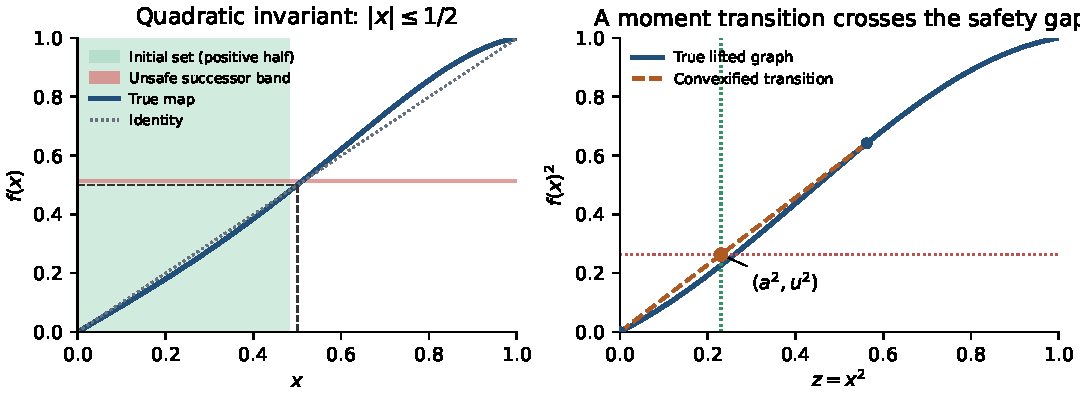
\includegraphics[width=.94\textwidth]{geometry.pdf}
\caption{Symmetric degree-gap example on its positive half. Left: $[-1/2,1/2]$ is invariant and excludes the unsafe band. Right: the chord from $(0,0)$ to $(t^2,f(t)^2)$ passes through $(a^2,u^2)$ in second-moment coordinates. Symmetric distributions cancel odd moments. The plot illustrates exact identities and is not proof of nonexistence.}\label{fig:moment}
\end{figure*}
\subsection{Scalar comparison degree two versus vector degree one}\label{sec:adding}
We strengthen the original contracting-rotation example to a uniform neighborhood of nonlinear maps. Write
\[
\begin{gathered}
 X=\{x\in\R^2:\|x\|_2\leq1\},\\
 X_0=\{x:\|x\|_2\leq\tfrac14\},\qquad X_u=\{(\tfrac34,0)\},\\
 R=\begin{pmatrix}0&-1\\1&0\end{pmatrix},\qquad q=\tfrac9{10}.
\end{gathered}
\]
\begin{proposition}[A perturbation-stable benefit from more affine functions]\label{prop:nonlinear}
Let $f:X\to\R^2$ be continuous and satisfy
\[
 f(x)=qRx+e(x),\qquad \sup_{x\in X}\|e(x)\|_2\leq\delta,\qquad 0\leq\delta<\tfrac1{20}.
\]
Then $f(X)\subseteq X$. At prescribed degree $d=1$, no scalar ordinary comparison certificate exists for any multiplier $\lambda\geq0$, whereas four affine components give a strict fixed-anchor VBC. The latter conclusion holds on the full convexified graph.
\end{proposition}
\begin{proof}
First, $\|f(x)\|_2\leq q+\delta<1$ on $X$.
Suppose a scalar affine certificate is $b(x)=a^\top x-c$.
Strict negativity at $0\in X_0$ gives $c>0$, and the unsafe condition implies
\[
 c<\tfrac34a_1\leq\tfrac34\|a\|_2,\qquad a\neq0.
\]
For $x_*=R^\top a/\|a\|_2\in X$, skew symmetry gives $a^\top x_*=0$, and hence
\[
 b(x_*)=-c<0,\qquad
 b(f(x_*))\geq(q-\delta)\|a\|_2-c>0,
\]
because $q-\delta>17/20>3/4$. This contradicts
$b\circ f\leq\lambda b$ for every $\lambda\geq0$.

For the four-component certificate put $r_0=1/2$ and
\[
\begin{gathered}
 G=\begin{pmatrix}1&0\\0&1\\-1&0\\0&-1\end{pmatrix},\qquad
 \Pi=\begin{pmatrix}0&0&0&1\\1&0&0&0\\0&1&0&0\\0&0&1&0\end{pmatrix},\\
 B(x)=Gx-r_0\one,\qquad A=q\Pi.
\end{gathered}
\]
Since $GR=\Pi G$, direct substitution yields
\[
 B(f(x))-AB(x)=Ge(x)-(1-q)r_0\one
 \leq-\bigl(\tfrac1{20}-\delta\bigr)\one.
\]
Every component is at most $-1/4$ on $X_0$, $B_1(3/4,0)=1/4$,
and $\rho(A)=q<1$. Affinity in $(s,t)$ extends the comparison from the graph to its full convex hull.
\end{proof}

\textbf{An explicit cubic family.}
For every $0<\theta\leq1/40$ take
\begin{equation}\label{eq:cubic-family}
 f_\theta(x)=\left[\tfrac9{10}-\theta(1-\|x\|_2^2)\right]Rx.
\end{equation}
Its degree is three, while the prescribed certificate degree remains one.
Here $e(x)=-\theta(1-\|x\|_2^2)Rx$ has norm at most $\theta$ on $X$,
so Proposition~\ref{prop:nonlinear} applies uniformly with $\delta=1/40$.
The same four affine functions and matrix certify every member of this family with
\[
 \delta_0=\delta_u=\tfrac14,\qquad \eta=\tfrac1{40},\qquad \rho(A)=\tfrac9{10}.
\]
This proves an actual nonlinear same-degree recovery. Four is an upper bound, not a proved minimum component count. The uniform perturbation proposition also shows that the recovery does not rely on one isolated polynomial identity.

\textbf{Increasing degree is an alternative.}
For the family \eqref{eq:cubic-family}, the scalar quadratic
\[
 b_2(x)=\|x\|_2^2-\tfrac14,\qquad A_2=[\tfrac{81}{100}]
\]
has $\|f_\theta(x)\|_2^2\leq(81/100)\|x\|_2^2$, because the radial factor in \eqref{eq:cubic-family} lies in $[7/8,9/10]$. Consequently
\[
 b_2(f_\theta(x))-\tfrac{81}{100}b_2(x)\leq-\tfrac{19}{400}.
\]
Its initial and unsafe margins are $3/16$ and $5/16$. Thus the minimum
scalar forward constant-comparison degree is exactly two, while the minimum degree
allowing a finite fixed-anchor VBC is exactly one: degree zero cannot separate
nonempty initial and unsafe sets. At degree one one must add functions;
increasing to degree two permits one function.

\textbf{The chosen-body hypothesis, including mixtures and both errors.}
For the cubic family use the uniform bound $\delta=1/40$. At $d=1$, a pair $(s,t)\in\mathcal F_1$ has
\[
 t=qRs+\bar e,\qquad\|\bar e\|_2\leq\delta,
\]
by averaging $e(x)$; it need not satisfy $t=f(s)$.
Set $C=[-1/2,1/2]^2$ and $\varepsilon=1/100$.
For every such pair, if $y=s+v\in C$ and
$\|v\|_2,\|w\|_2\leq\varepsilon$, then
\[
 \|t+w\|_\infty
 \leq qr_0+\delta+(q+1)\varepsilon
 \leq\tfrac{247}{500}<\tfrac12
 \qquad(\delta=1/40).
\]
Also $I_1+\varepsilon\ball\subseteq C$ and $C\cap J_1=\varnothing$.
This proves $T_\varepsilon(C)\subseteq C$ for all convexified transition pairs
and independent source/successor errors. Subsequent convex combinations remain in $C$.
The original linear rotation is the limiting case $e=0$, with the sharper
propagation margin $1/20$ and robust square bound $469/1000$.


\begin{table*}[t]
\centering
\caption{Proved degree and function-count comparisons. All VBC exclusions use a fixed anchor. Minimum degrees concern the entire stated class, not a selected numerical search.}\label{tab:comparisons}
\small
\begin{tabular}{@{}p{.23\textwidth}p{.34\textwidth}p{.18\textwidth}p{.17\textwidth}@{}}
\toprule
System & Established comparison & Direction & Spectral scope\\
\midrule
Symmetric scalar map and Theorem~\ref{th:family}
& Minimum implication degree $2$; minimum comparison degree $4$, at all finite counts.
& Forward and backward & Quartic $A=[1]$; forward Schur class excluded at every degree.\\
Cubic family \eqref{eq:cubic-family}
& Minimum scalar comparison degree $2$; minimum finite-vector degree $1$. One affine fails; four suffice.
& Forward & Explicit matrices are Schur stable; minimum affine vector count not claimed.\\
Extraction map $f=x/2+x^2/4$
& One affine suffices. Twelve quadratic components validate extraction from supplied body data.
& Forward & Scalar $A=[1/2]$; vector $\|A\|_\infty=58/125$.\\
\bottomrule
\end{tabular}
\end{table*}
\section{A Supplied-Body Extraction Example}\label{sec:nonlinear}
Take
\[
\begin{gathered}
 X=[-1,1],\qquad f(x)=\tfrac12x+\tfrac14x^2,\\
 X_0=[-\tfrac14,\tfrac14],\quad X_u=[\tfrac7{10},\tfrac45],\quad d=2.
\end{gathered}
\]
Since $f'(x)=(1+x)/2\in[0,1]$, $f(X)=[-1/4,3/4]\subseteq X$.
\textbf{Scalar baseline.}
A single affine function already certifies this system:
\[
\begin{gathered}
 b(x)=x-\tfrac35,\qquad A_{\rm sc}=[\tfrac12],\\
 b(f(x))-\tfrac12 b(x)=\tfrac14x^2-\tfrac3{10}\leq-\tfrac1{20}.
\end{gathered}
\]
Its initial and unsafe margins are respectively $7/20$ and $1/10$.
It belongs to the degree-at-most-two class and even has degree one.
Consequently the twelve-function construction below validates conditional extraction from a supplied certified body, but gives no advantage in function count, degree, or propagation margin over this scalar certificate. Its largest uniform propagation margin $73/2500$ for the fixed twelve-function pair is smaller than the scalar margin $1/20$. Section~\ref{sec:adding} supplies a separate nonlinear example with a proved benefit from adding functions.

\textbf{Supplied body and certified extraction data.}

Use $\phi_2(x)=(x,x^2)$ and $z_c=0$. For \emph{every} pair $(s,t)\in\mathcal F_2$,
\[
 t_1=\tfrac12s_1+\tfrac14s_2,\quad
 0\leq t_2\leq\tfrac9{16}s_2,\quad s_2\geq0.
\]
These follow by averaging the graph equalities and the pointwise bound
$f(x)^2=x^2(1/2+x/4)^2\leq(9/16)x^2$.
Consequently,
\[
 \|t\|_2^2\leq
 \left(\tfrac14+\tfrac1{16}+\tfrac{81}{256}\right)\|s\|_2^2
 =\tfrac{161}{256}\|s\|_2^2
 \leq(\tfrac{13}{16})^2\|s\|_2^2.
\]
This is a bound on mixed transition pairs, not just individual trajectories.

Let $C=(3/5)\mathbb B_2$, $\varepsilon=1/20$, and $\gamma=1/10$, with anchor $a_1=(1,0)$. On $I_2$,
$\|s\|_2\leq5/16$, so $I_2+\varepsilon\mathbb B_2\subseteq C$.
For any perturbed source $y=s+e\in C$ and independent successor error $w$, with $\|e\|_2,\|w\|_2\leq\varepsilon$,
\[
 \|t+w\|_2\leq\tfrac{13}{16}(3/5+\varepsilon)+\varepsilon
 =\tfrac{37}{64}<\tfrac35,
\]
leaving the certified inclusion gap $7/320$. The anchor strictly separates $J_2$ by $\gamma$. Thus the full robust convexified hypothesis holds. Notice that $f(1)=3/4\in X_u$; global avoidance in a single step is not assumed.

Here $r=2$ and $R/\varepsilon=12$. The direct support-net bound is $m\leq1537$, while Proposition~\ref{prop:projection} improves it to $m\leq112$: the expression inside its ceiling is $64\sqrt3$, between $110$ and $111$. Projection onto this ball is explicit. A smaller certified construction uses twelve rational unit normals, all with exact offset $3/5$:
\[
 \begin{gathered}
 a_1=(1,0),\quad a_2=(0,1),\\
 a_3=(-1,0),\quad a_4=(0,-1),\\
 a_5=(3/5,4/5),\quad a_6=(3/5,-4/5),\\
 a_7=(-3/5,4/5),\quad a_8=(-3/5,-4/5),\\
 a_9=(4/5,3/5),\quad a_{10}=(4/5,-3/5),\\
 a_{11}=(-4/5,3/5),\quad a_{12}=(-4/5,-3/5).
 \end{gathered}
\]
For $P=\{a_i^\top z\leq3/5\}$, exact two-facet vertex enumeration gives
$\max_{z\in P}\|z\|_2^2=2/5<(13/20)^2$, so \eqref{eq:otherpoly} holds. This is a direct geometric certificate; these twelve normals are not claimed to be the much finer universal net.

At the graph pair $(0,0)$, all facets equal $-3/5$, so nominal dual rows with margin $\varepsilon$ have row sums at most $11/12$. We may therefore take the sharper LP cap $\Lambda=1$.
Use the 161 exact nodes $x_\ell=-1+\ell/80$, $\ell=0,\ldots,160$.
Their covering radius is $h=1/160$. The derivative estimates
\[
\begin{aligned}
 \|\phi_2'(x)\|_2^2&=1+4x^2\leq5<3^2,\\
 \|(\phi_2\circ f)'(x)\|_2^2
 &=f'(x)^2(1+4f(x)^2)\\
 &\leq13/4<2^2.
\end{aligned}
\]
give $\xi_s=3/160$, $\xi_t=1/80$, and
$\xi_t+\Lambda\xi_s=1/32$.
LP discovery used target $1/80$; exact replay accepts the target
$\eta_*=1/100$ with minimum LP slack $1/400$.

Specifically, for $B_i(x)=a_{i1}x+a_{i2}x^2-3/5$, take the matrix with only
\[
 A_{1,5}=28/125,\qquad A_{5,5}=52/125,\qquad A_{9,5}=58/125
\]
nonzero. The finite constraints \eqref{eq:lp} hold exactly at all 161 nodes. Theorem~\ref{th:lp} certifies the global continuum inequalities, including every convexified transition pair, with
\[
\begin{gathered}
 \delta_0\geq\tfrac{23}{80},\qquad \delta_u\geq\tfrac1{10},\qquad
 \eta\geq\tfrac1{100},\\
 \rho(A)\leq\|A\|_\infty=\tfrac{58}{125}<1.
\end{gathered}
\]
This example verifies finite certificate extraction from the supplied certified body and cover. The scalar baseline above establishes that multiple components and degree two are unnecessary for safety of this particular system.

\textbf{Independent exact continuum check.}
For the same fixed $B,A$, expand the twelve polynomials
$r_i(x)=(AB(x))_i-B_i(f(x))$ in the degree-four Bernstein basis on $[-1,1]$:
\[
 r_i(2u-1)=\sum_{k=0}^4 c_{ik}\binom4k u^k(1-u)^{4-k},
 \qquad 0\leq u\leq1.
\]
For $r_i(2u-1)=\sum_{j=0}^4 q_{ij}u^j$, the conversion is
\[
 c_{ik}=\sum_{j=0}^k q_{ij}\frac{\binom{k}{j}}{\binom{4}{j}}.
\]

Exact rational conversion gives $\min_{i,k}c_{ik}=73/2500$. The basis functions are nonnegative and sum to one, so $r_i(x)\geq73/2500$ on the entire interval, independently of the cover/Lipschitz argument. Moreover $r_1(1)=73/2500$; this is the exact largest uniform global propagation margin for this \emph{fixed} certificate pair. It is not an optimum over other functions or matrices. The LP guarantee remains the conservative $1/100$ after charging the feature-cover errors. The replay records all sixty Bernstein coefficients and checks both proofs.

\subsection{Physical robustness is a different premise}\label{sec:physical}
Consider the nonidentity map
\[
\begin{gathered}
 X=[-1,1],\qquad f(x)=x^2,\\
 X_0=[-1/4,1/4],\qquad X_u=[3/4,1].
\end{gathered}
\]
The ordinary certificate $B(x)=x^2-1/2$, $A=[1]$ has
\[
\begin{gathered}
 B\leq-7/16\ \text{on }X_0,\qquad B\geq1/16\ \text{on }X_u,\\
 B(f(x))-B(x)=x^4-x^2\leq0\quad(x\in X).
\end{gathered}
\]
Yet $1\in X_u$ is a fixed point. No strict or Schur-stable fixed-anchor VBC exists at any degree or finite component count. By Theorem~\ref{th:main}, the robust convexified-feature hypothesis fails at every prescribed degree.

In contrast, additive \emph{state} disturbances $|d_k|\leq1/8$ preserve the safe interval $C_{\rm state}=[-1/2,1/2]$, because
\[
 f(C_{\rm state})+[-1/8,1/8]=[-1/8,3/8]\subseteq C_{\rm state}.
\]
This interval contains $X_0$ and avoids $X_u$, proving physical robust safety. Independent source and successor feature errors can move off the realizable monomial variety; they encode a different and stronger requirement in this example.

The original identity example gives the same ordinary-versus-strict distinction at degree one: $f(x)=x$ on $X=[-1,1]$, $X_0=[-1/2,0]$, $X_u=[1/2,1]$, and $B(x)=x-1/4$, $A=[1]$ satisfy ordinary separation and propagation. Every $\varepsilon>0$ allows successive feature increments of size at most $\varepsilon$ from $0$ to $1/2$, so $\mathcal K_\varepsilon$ reaches $J_1$.


\section{Exact Verification and Reproducibility}\label{sec:reproduction}
The default replays use only Python's standard library and exact rational arithmetic. The verification code, input data, tests and illustrative figure source are pinned to repository revision
\begin{center}\small\texttt{7b2d025abdf9786f55819a36b10ffd8a5e343375}.\end{center}
This evidence revision is available in the public artifact \cite{artifact}. From its checkout run:
\begin{verbatim}
python src/exact_verify.py
python src/exact_verify_converse.py
python src/constructive_converse.py
python -m unittest discover -s tests -v
\end{verbatim}
The observed statuses are \texttt{EXACT\_EVIDENCE\_VERIFIED}, \texttt{EXACT\_FINITE\_EVIDENCE\_VERIFIED}, and \texttt{EXACT\_CONSTRUCTIVE\_EVIDENCE\_VERIFIED}; all 20 tests pass. The three committed JSON reports reproduce byte-for-byte. Assertion-based scripts reject optimized Python mode; run without \texttt{-O}.

The first replay checks supports, probabilities, moments, invariant-domain identities, endpoint margins, and the quartic factorization. The second checks the scalar baseline, cubic-family polynomial identities and nonnegative disk factors, mixed-transition robustness, and rotation/moment data. The third checks the supplied-body polygon, 161 exact paired-cover nodes, all 1,932 LP inequalities, and an independent Bernstein proof of all twelve global residuals. The derivative and cover bounds, not node sampling alone, certify the continuum.

Tests reject incorrect moments, negative weights or matrix entries, wrong supports or rotation coupling, excessive margins, and understated feature-cover budgets. Optional SciPy discovery proposes a matrix, followed by rational reconstruction and exact checks. Infeasibility on a chosen grid is not proof of nonexistence elsewhere. The figure is illustrative. General theorems are mathematical proofs, not claimed proof-assistant formalizations. No new application-scale performance or SOS benchmark study is reported.

\section{Conclusion}
Function count and degree address different restrictions in safety certificates. A verified moment witness excludes every finite same-degree fixed-anchor comparison family. Robust separation of the full convexified monomial relation instead characterizes finite prescribed-degree forward VBCs with Schur-stable matrices. From a supplied certified convex body and effective support/cover data, finite facets and row LPs extract a certificate with explicit margins.

The two exact degree comparisons have different meanings. The symmetric example separates implication conditions from comparisons, with minima two and four. The cubic family separates scalar from vector comparisons, with minima two and one. They establish formulation-selection implications, not a complete automatic decision procedure. The general neutral-class converse, automatic body discovery, broader pointwise separation, and optimal component counts remain future directions.

\begin{thebibliography}{12}
\bibitem{vector} A. Sogokon, K. Ghorbal, Y. K. Tan, and A. Platzer, ``Vector Barrier Certificates and Comparison Systems,'' FM, LNCS 10951, pp. 418--437, 2018. \href{https://doi.org/10.1007/978-3-319-95582-7_25}{doi:10.1007/978-3-319-95582-7\_25}. Continuous-time foundations; distinct from the discrete-time definition used here.
\bibitem{ibc} M. A. Oumer, V. Murali, A. Trivedi, and M. Zamani, ``Safety Verification of Discrete-Time Systems via Interpolation-Inspired Barrier Certificates,'' IEEE Control Systems Letters, vol. 8, pp. 3183--3188, 2024. \href{https://doi.org/10.1109/LCSYS.2024.3521356}{doi:10.1109/LCSYS.2024.3521356}.
\bibitem{submission} R. Iraji, V. Murali, and M. Zamani, ``Duality and Complementarity of Vector and Interpolation-Inspired Barrier Certificates for Safety Verification: Toward Reduced Conservatism and Complexity,'' submitted manuscript, 2026. Version supplied as SCL-D-26-00958.
\bibitem{anand} M. Anand, R. Jungers, M. Zamani, and F. Allgower, ``On the Completeness and Ordering of Path-Complete Barrier Functions,'' \href{https://arxiv.org/abs/2503.19561}{arXiv:2503.19561v1}, 2025. Comparison uses this preprint version; accepted in Automatica, 2026.
\bibitem{pccc} R. Iraji, F. Galarza-Jimenez, and M. Zamani, ``Formal Verification of Switched Systems via Path-Complete Closure Certificates,'' supplied IEEE Control Systems Letters accepted author manuscript, 2026. \href{https://doi.org/10.1109/LCSYS.2026.3739034}{doi:10.1109/LCSYS.2026.3739034}.
\bibitem{hst} Z. Horv\'ath, Y. Song, and T. Terlaky,
\emph{Invariance Conditions for Nonlinear Dynamical Systems},
arXiv:1607.01107v1, 2016. Theorem 3.10 and Remark 3.11.
\par\url{https://arxiv.org/abs/1607.01107}.
\bibitem{liu} J. Liu, \emph{Converse Barrier Functions via Lyapunov Functions},
IEEE Transactions on Automatic Control, vol. 67, no. 1, pp. 497--503, 2022.
DOI: 10.1109/TAC.2021.3085419.
\par\url{https://arxiv.org/abs/2007.11086}.
\bibitem{cone2024} G. O. Berger, M. Ghanbarpour, and S. Sankaranarayanan,
\emph{Cone-Based Abstract Interpretation for Nonlinear Positive Invariant Synthesis},
Proceedings of HSCC '24, pp. 1--16, 2024.
DOI: 10.1145/3641513.3650127.
\par\url{https://guberger.github.io/assets/papers/10.1145_3641513.3650127.pdf}.
\bibitem{harpeled} S. Har-Peled and M. Jones,
\emph{A Proof of Dudley's Convex Approximation},
arXiv:1912.01977v3, 2024. Theorem 1.4.
\par\url{https://arxiv.org/abs/1912.01977v3}.
\bibitem{alessio} A. Alessio, M. Lazar, A. Bemporad, and W. P. M. H. Heemels,
\emph{Squaring the circle: An algorithm for generating polyhedral invariant sets from ellipsoidal ones},
Automatica, vol. 43, no. 12, pp. 2096--2103, 2007.
DOI: 10.1016/j.automatica.2007.04.028.
\par\url{https://cse.lab.imtlucca.it/~bemporad/publications/papers/automatica_squaring_circle.pdf}.
\bibitem{berger} G. O. Berger and S. Sankaranarayanan,
\emph{Counterexample-guided computation of polyhedral Lyapunov functions for piecewise linear systems},
Automatica, vol. 155, article 111165, 2023.
DOI: 10.1016/j.automatica.2023.111165.
\bibitem{artifact} R. Iraji, \emph{Certificate Expressiveness: exact verification artifact}, repository revision 7b2d025abdf9786f55819a36b10ffd8a5e343375, 2026.
\par\url{https://github.com/rezairaji60/certificate-expressiveness/tree/7b2d025abdf9786f55819a36b10ffd8a5e343375}.
\end{thebibliography}
\end{document}
